\documentclass[a4j]{jarticle}			% for platex
\usepackage[dvipdfmx]{graphicx}
\usepackage{multicol}
\usepackage{mathtools}
\usepackage{amsmath, amssymb, amsfonts}


\title{未タイトル}
\author{学籍番号 20C1119 森田大雅}
\date{\today}

\begin{document}
\maketitle % タイトルなどの出力
\normalsize

% \twocolumnは二段組ににしない文章

\begin{abstract}
描画ロボットの研究において、輪郭$\lparen\text{エッジ}\rparen$抽出を行って鉛筆画やハッチング$\lbrack1\rbrack$、インクイラストなどの芸術表現に応用する研究$\lbrack2\rbrack$や機械に手順を示し、そのとおりに描かせる研究$\lbrack3\rbrack$が存在する.
しかし、実際に$\lceil \text{人が描くような描き方} \rfloor$を追求したものは少ないと感じた.
そこで、今回はキャラクターの画像から線画を描く、そしてできるだけ人が描いたような描き方をする描画ロボットを作成する.
\end{abstract}

\begin{multicols}{2} %二段組にする

\section{introduction}
描画ロボットにおいてプロッターやそれに似た機構で絵を描かせる研究や開発は多く見られるが、人の腕に似た機構であるロボットアームを用いて絵を描かせる研究はあまり存在しない.
じつは現代の美術の人物などのデッサンにおいては輪郭を明確に描くやり方はあまり取らない.
それは古典的なやり方で、昔の巨匠が実際そのように描くことは普通だった.
今でも意図的な理由があって、輪郭を描くことである表現をしたい場合に使うことは確かにある.
人に似たのような描き方をさせたいという以上、輪郭やどこから描くなどの描き順に拘りたい所ではあるが、描き順のパターンを機械学習に任せて描かせることなども含めて行うのは難易度がかなり高い.
そこで今回は3軸のロボットアームで、一枚の画像の輪郭を抽出し、人が描くような描き方を考えたい.
線の経路を求める方法は現時点で2通り考えている. 
一方が左上から右下へ走査していき、線の画素を見つける度にたどるラスタスキャンの方法である. 
もう一方は端点を持つ線から描いていく方法である.
ただしこちらはスタート地点をランダムにしており、場合によっては1.1の手順とは程遠くなってしまうことがある. 
しかし直感的にラスタスキャンより端点から描くほうが人が描いたように見えると考えたため、今回用いることにした.

\subsection{人のような描き方の定義}
本研究では$\lbrack4\rbrack$を参考に描き方の方針を進めている.
顔のパーツ配置が定まりやすいという部分に焦点を当てた.\\
描き順としては顎や髪、頭などの頭上部から描き、次に目や鼻、耳などの細部を描く.
理由は全体を描いてから、細部を描いた方が目や鼻の位置を定めやすいからである.

\section{システム構成}
\subsection{Hardware}


\subsection{Image Processing}
前処理として任意の一枚の画像をガウシアンフィルタで平滑化、エッジ抽出、Zhang-Suenで細線化を行っている.\\ 
エッジ抽出に関しては、OpenCVのガウシアンフィルやCannyで処理した後に細線化処理を施すと線が途切れたり、ノイズが現れてしまう.
そこでCannyのエッジ検出器を向上させる"Enhanced Edge Detection Using SR-Guided Threshold Maneuvering and Window Mappinf: Haneding Broken Edges and Noisy Structures in Canny Edge"という論文とOpenCVのラプラシアンフィルタとCannyの3つを比較した.
結果として、\underline{ooo}を用いることに決めた.
後に3つの比較実験を示す.
経路を辿るとき、2つの方法を考えた.
一方は、左上から右下へ走査するラスタスキャンを用いる方法である.
もう一方は、前処理で出力された画像から端点を検出し、端点を持つ線から描いていく方法である.
理由は端点を持つ線から描くほうが人が描いたように見えると直感的に考えたからである.
線の経路の求め方は、ある線の画素から隣に線の画素があるかを探して、移動してを繰り返すものとなっている.
そのため、線を一本に単純化してある方が線をたどるのに容易であるため細線化を行う.

 % \subsection{線のたどり方}  概要なので割愛

\subsection{端点を持つ線から描く理由}
端点を検出して描くのには2つの理由がある.
線画を生成する過程で繋がっているはずの線が途切れてしまうというのが一つの理由である.
それは平滑化、エッジ抽出、細線化処理を施すからである.

\end{multicols}
\section{ロボットの機構}
本研究で用いるロボットは3軸のマニピュレータロボットである.
下の図1のようにアームの先端、姿勢の関節角を$\theta_1, \theta_2, \theta_3$、各リンクの長さ$l_1, l_2, l_3, l_4$とし、逆運動学問題を解く.
またリンク座標系を定める方法として、DH記法(Denavit-Hartenberg記法)を用いる.


\begin{figure}[htbp]
\begin{center}
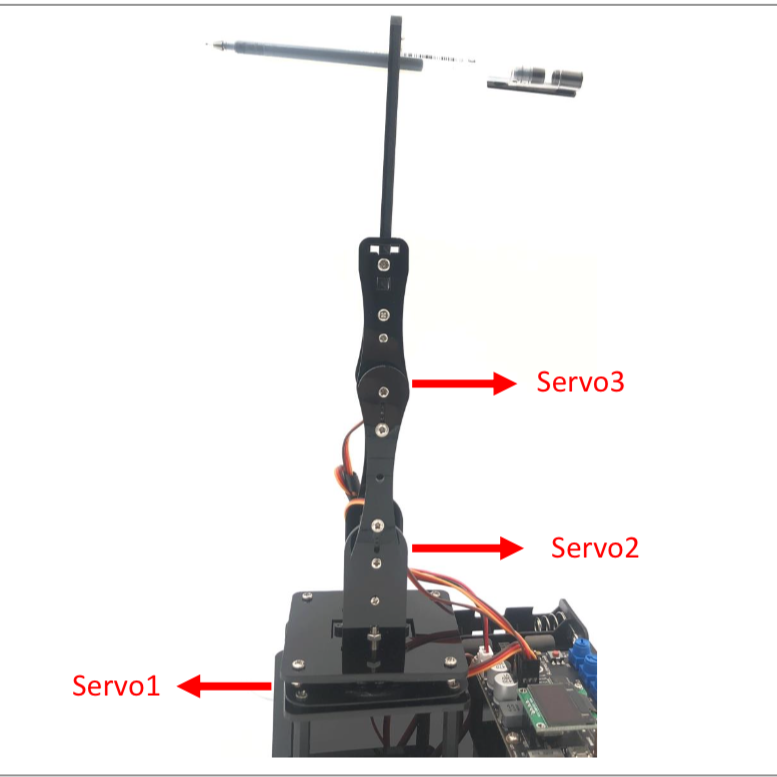
\includegraphics[width=80mm]{/home/morita/ros2_ws/Memo/tex/img/IMG_0025.PNG}
\caption{実機}
\end{center}
\end{figure}


\section{手先の位置と回転角の関係}

運動学、逆運動学を用いて、ペン先の位置を各サーボモータの回転角を導出する.
リンク座標系は以下のように定義する.
\begin{figure}[htbp]
\begin{center}
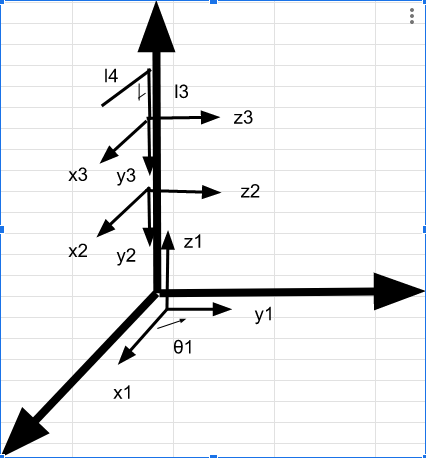
\includegraphics[width=75mm]{/home/morita/ros2_ws/Memo/tex/img/link.png}
\caption{リンク座標系}
\end{center}
\end{figure}

\begin{multicols}{2} %二段組にする

座標系0から3への座標変換行列 
\small
$$
	^{0}T_{3}=^{0}T_{1} ^{1}T_{2} ^{2}T_{3} \\
$$
\begin{equation*}
	\begin{array}{cc}
		=
		\left( 
			\begin{array}{cccc}
				C_1C_{23} & -C_1S_{23} & 0 & l_2C_1S_2 \\
				S_1C_{23} & -S_1S_{23} & 0 & l_2S_1S_2 \\
				-S{23} & -C_{23} & -1 & l_2C_2 + l_1 \\
				0 & 0 & 0 & 1 
			\end{array}
		\right)
	\end{array}
\end{equation*}
\normalsize
ただし、
\begin{equation*}
	\left(
	\begin{split}
		C_{23} = cos\theta_2cos\theta_3-sin\theta_2sin\theta_3\\
		S_{23} = sin\theta_2cos\theta_3+cos\theta_2sin\theta_3	
	\end{split}
	\right)
\end{equation*}
\normalsize
手先ベクトル
\tiny
\begin{equation*}
	\begin{array}{cccc}
		&\left( 
			\begin{array}{cccc}
				1 & 0 & 0 & l_4\\
				0 & 1 & 0 & 0\\
				0 & 0 & 1 & 0\\
				0 & 0 & 0 & 1 
			\end{array}
		\right)
		\left( 
			\begin{array}{cccc}
				1 & 0 & 0 & 0\\
				0 & 1 & 0 & -l_3\\
				0 & 0 & 1 & 0\\
				0 & 0 & 0 & 1 
			\end{array}
			\right)\\
		&=
		\left( 
		\begin{array}{cccc}
			1 & 0 & 0 & l_4\\
			0 & 1 & 0 & -l_3\\
			0 & 0 & 1 & 0\\
			0 & 0 & 0 & 1 
		\end{array}
		\right)
	\end{array}
\end{equation*}
\normalsize
より手先までの座標変換行列$^{0}P_{r}$が以下のように求まる.
\tiny
\begin{equation*}
	\begin{array}{cc}
		\left( 
			\begin{array}{cccc}
				C_1C_{23} & -C_1S_{23} & 0 & l_4C_1C_{23}+l_3C_1S_{23}+l_2C_1S_2 \\
				S_1C_{23} & -S_1S_{23} & 0 & l_4S_1C_{23}+l_3S_1S_{23}+l_2S_1S_2 \\
				-S{23} & -C_{23} & -1 & -l_4S_{23}+l_3C_{23}+l_2C_2+l_1 \\
				0 & 0 & 0 & 1 
			\end{array}
		\right)
	\end{array}
\end{equation*}
\small
そしてこの行列から手先の位置x, y, zは以下のように求まる.
\begin{equation}
	\left\{
		\begin{array}{c}
		\begin{split}
			&x=C_1(l_4C_{23}+l_3S_{23}+l_2S_2)\quad(3.1) \\
			&y=S_1(l_4C_{23}+l_3S_{23}+l_2S_2)\quad(3.2) \\
			&z-l_1=-l_4S_{23}+l_3C_{23}+l_2C_2\quad(3.3) \\
		\end{split}
	\end{array}
	\right.
\end{equation}
これらの逆運動学を解くと
\tiny
\begin{equation}
	\left\{
		\begin{array}{c}
		\begin{split}
			\theta_1&=\frac{1}{2}cos^{-1}\biggl( \frac{x^2-y^2}{x^2+y^2} \biggr) \\
			\theta_2&= cos^{-1}\biggl( \frac{x^2+y^2+(z-l1)^2+l_2^2-l_3^2-l_4^2}{2l_    2\sqrt{x^2+y^2+(z-l_1)^2}} \biggr)\\
			&\qquad\qquad+tan^{-1}\biggl( \frac{\sqrt{x^2+y^2}}{z-l1}\biggr) \\
			\theta_3&=cos^{-1}\biggl( \frac{x^2+y^2+(z-l1)^2-l_4^2-l_3^2-l_2^2}{2l_2    \sqrt{l_3^2+l_4^2}}\biggr)\\
			&\qquad\qquad+tan^{-1}\biggl( \frac{-l_4}{l_3}\biggr)\\
		\end{split}
		\end{array}
	\right.
\end{equation}
\normalsize

\section{手先の到達範囲}
描画は第一象限で行うこととする.
この条件と不等式にまとめると以下のようになる.
\small
\begin{equation*}
	\left\{
		\begin{array}{c}
			\begin{split}
				&0 \leqq \theta_1 \leqq \frac{\pi}{2} & \\
				&x \geqq 0 \land y \geqq 0
			\end{split}
		\end{array}
	\right.
\end{equation*}
\normalsize
手先の最大到達点は
\small
\begin{equation*}
	l_2+l_3=65+130=195
\end{equation*}
\normalsize
また、第一象限に描きたいが、手先が一回転するのは避けたい.
それはつまり、$\theta_2\geqq0\ (\land)\ \theta_3\geqq0$ということである.
逆運動学解の$\theta_3$を用いると、$-1\leqq cos((\theta_3-\alpha)\leqq 1)$より
\small
\begin{equation*}
	-2l_2\sqrt{l_3^2+l_4^4}-(z-l_1)^2+(l_4^2+l_3^2+l_2^2)\leqq x^2+y^2\leqq 195
\end{equation*}
$$
	(\text{最左辺})=116.4208\cdots
$$
\normalsize
よって求めたい手先の範囲は以下のようになる.
\small
\begin{equation*}
	\therefore\ 117 \leqq x^2+y^2 \leqq 195
\end{equation*}
\normalsize
	
\section{実験}
\subsection{エッジ}
\subsection{端点とラスタスキャン}
今回は端点を持つ線から描く場合と、ラスタスキャンで線の経路を求めた場合を比較し、より人らしい描き方の方を用いる.
どちらが人のような描き方に近いかアンケートをx人にとる.
\section{出力結果}

以下に今回使用した実機で端点から描いたものと、ラスタスキャンで求めた経路をもとに機械に描かせた画像を載せる.

\section{参考文献}

\begin{enumerate}
\item \lbrack 1\rbrack \ Raspberry Piを利用した肖像画描画ロボット :$ \lceil Pankraz Piktograph \rfloor$ 
\item \lbrack 2\rbrack \ XDoG: An Xtended difference-of-Gaussians compendium
\item \lbrack 3\rbrack \ ロボットによる描画行為の再現
\item \lbrack 4\rbrack \ 出版:主婦の友社\ $\lceil \text{小河原智子の似顔絵入門} \rfloor$
\item 広瀬\ 茂男\ 著\ 機械工学選書\ 裳華房\ ロボット工学-機械システムのベクトル解析-
\item 細田\ 耕著\ 実践ロボット制御-基礎から動力学まで-
\item \ "Enhanced Edge Detection Using SR-Guided Threshold Maneuvering and Window Mapping: Haneding Broken Edges and Noisy Structures in Canny Edge"
\end{enumerate}

\end{multicols}

\end{document}
